\documentclass{beamer}
\beamertemplatenavigationsymbolsempty % remove the default navigation symbols
% default colors
% used in standalone pictures and when no university is selected
\definecolor{black}{HTML}{000000}
\definecolor{green}{HTML}{33BB33}
\definecolor{red}{HTML}{BB3333}
\definecolor{orange}{HTML}{BB6600}
\definecolor{blue}{HTML}{3333BB}
\definecolor{uulmaccent}{HTML}{999999}

\definecolor{uulmlogoblue}{named}{blue}
\definecolor{uulmblue}{named}{blue}

\ifdarkmode
	\colorlet{green}{green!85!white}
	\colorlet{red}{red!85!white}
	\colorlet{orange}{orange!85!white}
	\colorlet{blue}{blue!85!white}
	\setbeamercolor{section in toc shaded}{fg=black}
	\setbeamertemplate{section in toc shaded}[default][50]
\fi


\makeatletter
    \setlength\beamer@paperwidth{100mm}%
    \setlength\beamer@paperheight{80mm}%
    \geometry{papersize={\beamer@paperwidth,\beamer@paperheight}}
\makeatother
\setbeamersize{text margin left=0mm,text margin right=0mm}

\usepackage{tikz}
\usetikzlibrary{arrows.meta}

\newcommand{\graph}[4]{
	\centering
	\begin{tikzpicture}[xscale=2,yscale=2,line width=3pt,every node/.style={inner sep=0pt},node/.style={shape=circle,draw,minimum size=10mm},weight/.style={inner sep=3pt,white,#2},edge/.style={shorten <= 5pt,shorten >= 5pt,#1},oedge/.style={edge,#3}]
		\only<2->{\node at (-.5,-.7) {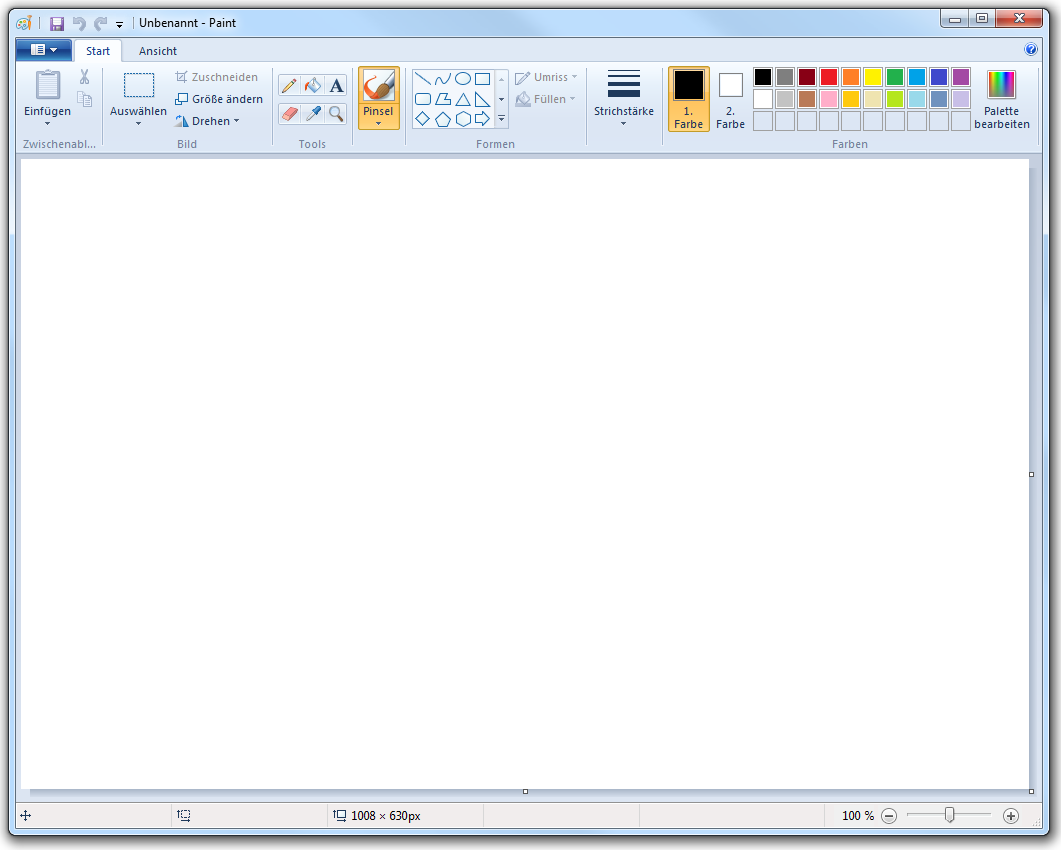
\includegraphics[width=\linewidth]{paint}};}
		\node[node,name=n1,fill=blue!50!white,#4] at (0,0) {};
		\node[node,name=n2,fill=red!50!white,#4] at (-1,-2) {};
		\node[node,name=n3,fill=yellow!50!white,#4] at (1,-2) {};
		\node[node,name=n4,fill=green!50!white,#4] at (-2,0) {};
		\draw[oedge] (n1) -- node[weight,above left]  {\Huge\textbf{2}} (n2);
		\draw[oedge] (n2) -- node[weight,above]       {\Huge\textbf{1}} (n3);
		\draw[edge]  (n1) -- node[weight,above right] {\Huge\textbf{6}} (n3);
		\draw[oedge] (n4) -- node[weight,above]       {\Huge\textbf{3}} (n1);
	\end{tikzpicture}
}

\begin{document}

	\begin{frame}[plain]
		\graph{}{}{}{fill=white}
	\end{frame}

	\begin{frame}[plain]
		\graph{->}{}{}{fill=white}
	\end{frame}

	\begin{frame}[plain]
		\graph{}{black}{}{fill=white}
	\end{frame}

	\begin{frame}[plain]
		\graph{->}{black}{}{fill=white}
	\end{frame}

	\begin{frame}[plain]
		\graph{->}{black}{blue}{fill=white}
	\end{frame}

	\begin{frame}[plain]
		\graph{}{}{}{}
	\end{frame}

	\begin{frame}[plain]
		\graph{->}{}{}{}
	\end{frame}

	\begin{frame}[plain]
		\graph{}{black}{}{}
	\end{frame}

	\begin{frame}[plain]
		\graph{->}{black}{}{}
	\end{frame}

	\begin{frame}[plain]
		\graph{->}{black}{blue}{}
	\end{frame}

	\begin{frame}[plain]
		\graph{shorten <= 0pt,shorten >= 0pt}{}{}{fill=white}
	\end{frame}

	\begin{frame}[plain]
		\graph{shorten <= 0pt,shorten >= 0pt,->}{}{}{fill=white}
	\end{frame}

	\begin{frame}[plain]
		\graph{shorten <= 0pt,shorten >= 0pt}{black}{}{fill=white}
	\end{frame}

	\begin{frame}[plain]
		\graph{shorten <= 0pt,shorten >= 0pt,->}{black}{}{fill=white}
	\end{frame}

	\begin{frame}[plain]
		\graph{shorten <= 0pt,shorten >= 0pt,->}{black}{blue}{fill=white}
	\end{frame}

	\begin{frame}[plain]
		\graph{shorten <= 0pt,shorten >= 0pt}{}{}{}
	\end{frame}

	\begin{frame}[plain]
		\graph{shorten <= 0pt,shorten >= 0pt,->}{}{}{}
	\end{frame}

	\begin{frame}[plain]
		\graph{shorten <= 0pt,shorten >= 0pt}{black}{}{}
	\end{frame}

	\begin{frame}[plain]
		\graph{shorten <= 0pt,shorten >= 0pt,->}{black}{}{}
	\end{frame}

	\begin{frame}[plain]
		\graph{shorten <= 0pt,shorten >= 0pt,->}{black}{blue}{}
	\end{frame}

	\begin{frame}[plain]
		\graph{}{black}{blue}{fill=white}
	\end{frame}

	\begin{frame}[plain]
		\graph{}{black}{blue}{}
	\end{frame}

	\begin{frame}[plain]
		\graph{shorten <= 0pt,shorten >= 0pt}{black}{blue}{fill=white}
	\end{frame}

	\begin{frame}[plain]
		\graph{shorten <= 0pt,shorten >= 0pt}{black}{blue}{}
	\end{frame}

\end{document}
